%!TEX TS-program = xelatex
%!TEX encoding = UTF-8

% LaTeX source for the errata of the book ``代数学方法'' in Chinese
% Copyright 2018  李文威 (Wen-Wei Li).
% Permission is granted to copy, distribute and/or modify this
% document under the terms of the Creative Commons
% Attribution 4.0 International (CC BY 4.0)
% http://creativecommons.org/licenses/by/4.0/

% 《代数学方法》卷一勘误表 / 李文威
% 使用自定义的文档类 AJerrata.cls. 自动载入 xeCJK.

\documentclass{AJerrata}

\usepackage{unicode-math}

\usepackage[unicode, colorlinks, psdextra, bookmarksnumbered,
	pdfpagelabels=true,
	pdfauthor={李文威 (Wen-Wei Li)},
	pdftitle={代数学方法卷一勘误},
	pdfkeywords={}
]{hyperref}

\setmainfont[
	BoldFont={TeX Gyre Termes Bold},
	ItalicFont={TeX Gyre Termes Italic},
	BoldItalicFont={TeX Gyre Termes Bold Italic},
	PunctuationSpace=2
]{TeX Gyre Termes}

\setsansfont[
	BoldFont=FiraSans-Bold.otf,
	ItalicFont=FiraSans-Italic.otf
]{FiraSans-Regular.otf}

\setCJKmainfont[
	BoldFont=Noto Serif CJK SC Bold
]{Noto Serif CJK SC}

\setCJKsansfont[
	BoldFont=Noto Sans CJK SC Bold
]{Noto Sans CJK SC}

\setCJKfamilyfont{emfont}[
	BoldFont=FandolHei-Regular.otf
]{FandolHei-Regular.otf}	% 强调用的字体

\renewcommand{\em}{\bfseries\CJKfamily{emfont}} % 强调

\setmathfont[
	Extension = .otf,
	math-style= TeX,
]{texgyretermes-math}

\usepackage{mathrsfs}
\usepackage{stmaryrd} \SetSymbolFont{stmry}{bold}{U}{stmry}{m}{n}	% 避免警告 (stmryd 不含粗体故)
% \usepackage{array}
% \usepackage{tikz-cd}  % 使用 TikZ 绘图
\usetikzlibrary{positioning, patterns, calc, matrix, shapes.arrows, shapes.symbols}

\usepackage{myarrows}				% 使用自定义的可伸缩箭头
\usepackage{mycommand}				% 引入自定义的惯用的命令


\title{\bfseries 代数学方法(第一卷)勘误表}
\author{李文威}
\date{\today}

\begin{document}
	\maketitle
	以下页码等信息参照高等教育出版社 2019 年 1 月出版之《代数学方法》第一卷, ISBN: 978-7-04-050725-6. 这些错误将在新版一并改正.

	\begin{Errata}
		\item[第 12 页, 倒数第 8 行]
		\Orig 也可以由稍后的无穷公理保证.
		\Corr 也可以划入稍后的无穷公理.
		\Thx{感谢王东瀚指正.}
		
		\item[第 16 页, 定义 1.2.8]
		\Orig 若传递集 $\alpha$ 对于 $\in$ 构成良序集, 则称 $\alpha$ 为\emph{序数}.
		\Corr 若传递集 $\alpha$ 对于 $x < y \stackrel{\text{定义}}{\iff} x \in y$ 成为良序集, 则称 $\alpha$ 为\emph{序数}.
		\Thx{感谢王东瀚指正.}
		
		\item[第 16 页, 倒数第 5 行]
		\Orig 于是有 $\gamma \in \gamma$, 这同偏序的反称性矛盾.
		\Corr 于是有 $\gamma \in \gamma$, 亦即在偏序集 $(\alpha, \leq)$ 中 $\gamma < \gamma$, 这同 $<$ 的涵义 ($\leq$ 但 $\neq$) 矛盾.
		\Thx{感谢王东瀚指正.}
		
		\item[第 23 页, 第 5 行]
		\Orig 由于 $\sigma$ 无穷...
		\Corr 由于 $\aleph_\sigma$ 无穷...
		\Thx{感谢王东瀚指正.}
		
		\item[第 42 页, 倒数第 2 行]
		\Orig ...同构. $Z(\cdots) \simeq $...
		\Corr ...同构 $Z(\cdots) \simeq$...
		\Thx{感谢王东瀚指正.}
		
		\item[第 49 页, 倒数第 9 行]
		\Orig 由此得到伴随对 $(D^{\mathrm{op}}, D, \varphi)$.
		\Corr 由此得到伴随对 $(D^{\mathrm{op}}, D, \varphi^{-1})$.
		\Thx{感谢王东瀚指正.}
		
		\item[第 54 页最后] \Corr 图表微调成
		\begin{center}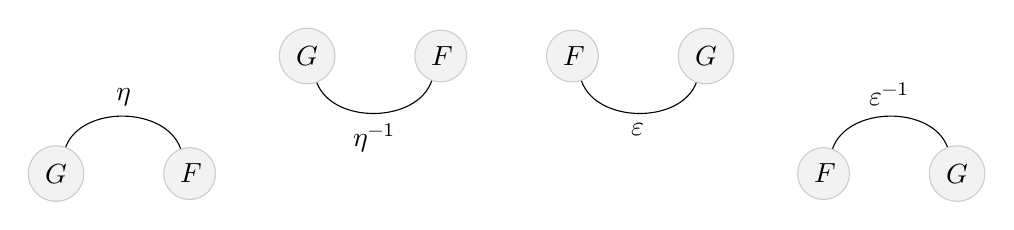
\begin{tikzpicture}[bend angle=70, auto, fct/.style={circle, draw=gray!40, fill=gray!10}]
			\node[fct] (G1) {$G$}; \node[fct] (F1) [right=of G1] {$F$} edge[bend right] node[swap] {$\eta$} (G1);
			\node[fct] (G2) [above right=of F1] {$G$}; \node[fct] (F2) [right=of G2] {$F$} edge[bend left] node {$\eta^{-1}$} (G2);
			\node[fct] (F3) [right=of F2] {$F$}; \node[fct] (G3) [right=of F3] {$G$} edge[bend left] node {$\varepsilon$} (F3);
			\node[fct] (F4) [below right=of G3] {$F$}; \node[fct] (G4) [right=of F4] {$G$} edge[bend right] node[swap] {$\varepsilon^{-1}$} (F4);
		\end{tikzpicture}\end{center}
		兴许更易懂. \Thx{感谢熊锐提供意见.}

        \item[第 94 页, 习题 5 倒数第 2 行]
        \Orig Yang--Baxter 方程.
        \Corr 杨--Baxter 方程.
        
        \item[第 116 页, 第 5 行]
        \Orig $\bar{H} \subseteq N_{\bar{G}}(\bar{H})$
        \Corr $\bar{H} \subsetneq N_{\bar{G}}(\bar{H})$

		\item[第 126 页, 第 6 行]
		\Orig $\left( \cdots \right)_{i=0}^n$
		\Corr $\left( \cdots \right)_{i=0}^{n-1}$

        \item[第 141 页, 第 11 行]
        \Orig 另外约定 $\mathfrak{S}'_n = \{1\}$
        \Corr 另外约定 $\mathfrak{S}'_1 = \{1\}$

		\item[第 149 页, 第 3 行]
		$\mathsf{CRing}$ 表交换环范畴. 另外此行应缩进.

		\item[第 165 页, 5.3.11 之上两行]
		\Orig $\exists s \in R$
		\Corr $\exists s \in S$

        \item[第 220 页]
        本页出现的 $\mathrm{Bil}(\bullet \times \bullet; \bullet)$ 都应该改成 $\mathrm{Bil}(\bullet, \bullet; \bullet)$, 以和 216 页的符号保持一致.
        
   		\item[第 205 页, 第 7 行]
        \Orig $M$ 作为 $R/\mathrm{ann}(M)$-模自动是无挠的.
        \Corr $M$ 作为 $R/\mathrm{ann}(M)$-模的零化子自动是 $\{0\}$.
        \Thx{感谢戴懿韡指正.}
        
        \item[第 228 页, 倒数第 4 行]
        \Orig $\sum_{y \in R}$
        \Corr $\sum_{y \in Y}$
        
        \item[第 246 頁, 第 16 行]
        \Orig $u_i f_i$
        \Corr $u_i \alpha_i$
        \Thx{感谢陆睿远指正.}
        
        \item[第 247 頁, 第 6---7 行]
        \Orig 其长度记为 $n+1$.
        \Corr 其长度定为 $n$.
        
        \item[第 264 頁, 第 14 行]
        \Orig 如果 $\mathrm{ann}(M) = \{0\}$
        \Corr 如果 $\mathrm{ann}(N) = \{0\}$
        
        \item[第 311 页, 命题 8.3.2 证明第 4 行]
        \Corr 分别取......和 $\overline{F}' | E'$.

        \item[第 315 页, 倒数第 2 行]
        \Orig $\deg f(X^p) = pf(X)$
        \Corr $\deg f(X^p) = p \deg f(X)$
        \Thx{感谢杨历指正.}
        
        \item[第 317 页, 倒数第 13 行]
        (出现两次)\;
        \Orig $\prod_{i=1}^n \cdots$
        \Corr $\prod_{m=1}^n \cdots$
        
        \item[第 359 页, 倒数第 2 行]
        \Orig $\in A_F$
        \Corr $\in A_E$
        \Thx{感谢杨历指正.}
        
        \item[第 360 页, 证明]
        将所有 $\chi(\cdots) = 1$ 改成 $\chi(\cdots) = 0$, 以确保与之前的惯例一致.
        \Thx{感谢杨历指正.}
	\end{Errata}
	
\end{document}